\documentclass[11pt,t]{beamer}
% xcolor and define colors -------------------------
\usepackage{xcolor}

% https://www.viget.com/articles/color-contrast/
\definecolor{purple}{HTML}{695693}
\definecolor{navy}{HTML}{567293}
\definecolor{ruby}{HTML}{9a2515}
\definecolor{alice}{HTML}{107895}
\definecolor{daisy}{HTML}{EBC944}
\definecolor{coral}{HTML}{F26D21}
\definecolor{kelly}{HTML}{829356}
\definecolor{cranberry}{HTML}{E64173}
\definecolor{jet}{HTML}{131516}
\definecolor{asher}{HTML}{555F61}
\definecolor{slate}{HTML}{314F4F}

% Main theme colors
\definecolor{accent}{HTML}{107895}
\definecolor{accent2}{HTML}{9a2515}

\newcommand\navy[1]{{\color{navy}#1}}
\newcommand\purple[1]{{\color{purple}#1}}
\newcommand\kelly[1]{{\color{kelly}#1}}
\newcommand\ruby[1]{{\color{ruby}#1}}
\newcommand\alice[1]{{\color{alice}#1}}
\newcommand\daisy[1]{{\color{daisy}#1}}
\newcommand\coral[1]{{\color{coral}#1}}
\newcommand\cranberry[1]{{\color{cranberry}#1}}
\newcommand\slate[1]{{\color{slate}#1}}
\newcommand\jet[1]{{\color{jet}#1}}
\newcommand\asher[1]{{\color{asher}#1}}

\newcommand\bgNavy[1]{{\colorbox{navy!80!white}{\textcolor{white}{#1}}}}
\newcommand\bgPurple[1]{{\colorbox{purple!80!white}{\textcolor{white}{#1}}}}
\newcommand\bgKelly[1]{{\colorbox{kelly!80!white}{\textcolor{white}{#1}}}}
\newcommand\bgRuby[1]{{\colorbox{ruby!80!white}{\textcolor{white}{#1}}}}
\newcommand\bgAlice[1]{{\colorbox{alice!80!white}{\textcolor{white}{#1}}}}
\newcommand\bgDaisy[1]{{\colorbox{daisy!80!white}{\textcolor{white}{#1}}}}
\newcommand\bgCoral[1]{{\colorbox{coral!80!white}{\textcolor{white}{#1}}}}
\newcommand\bgCranberry[1]{{\colorbox{cranberry!80!white}{\textcolor{white}{#1}}}}


% Beamer Options -------------------------------------

% Background
\setbeamercolor{background canvas}{bg = white}

% Change text margins
\setbeamersize{text margin left = 15pt, text margin right = 15pt} 

% \alert
\setbeamercolor{alerted text}{fg = accent2}

% Frame title
\setbeamercolor{frametitle}{bg = white, fg = jet}
\setbeamercolor{framesubtitle}{bg = white, fg = accent}
\setbeamerfont{framesubtitle}{size = \small, shape = \itshape}

% Block
\setbeamercolor{block title}{fg = white, bg = accent2}
\setbeamercolor{block body}{fg = jet, bg = jet!10!white}

% Title page
\setbeamercolor{title}{fg = jet}
\setbeamercolor{subtitle}{fg = accent}

%% Custom \maketitle and \titlepage
\setbeamertemplate{title page}
{
    %\begin{centering}
        \vspace{20mm}
        {\Large \usebeamerfont{title}\usebeamercolor[fg]{title}\inserttitle}\\ \vskip0.25em%
        \ifx\insertsubtitle\@empty%
        \else%
          {\usebeamerfont{subtitle}\usebeamercolor[fg]{subtitle}\insertsubtitle\par}%
        \fi% 
        {\vspace{10mm}\insertauthor}\\
        {\color{asher}\small{\insertdate}}\\
    %\end{centering}
}

% Table of Contents
\setbeamercolor{section in toc}{fg = accent!70!jet}
\setbeamercolor{subsection in toc}{fg = jet}

% Button 
\setbeamercolor{button}{bg = accent}

% Remove navigation symbols
\setbeamertemplate{navigation symbols}{}

% Optional: page numbers at bottom
\addtobeamertemplate{navigation symbols}{}{%
    \usebeamerfont{footline}%
    \hspace{1em}%
    \alice{\insertframenumber/\inserttotalframenumber}
    \vspace*{1.5mm}
}


% Table and Figure captions
\setbeamercolor{caption}{fg=jet!70!white}
\setbeamercolor{caption name}{fg=jet}
\setbeamerfont{caption name}{shape = \itshape}

% Bullet points

%% Fix left-margins
\settowidth{\leftmargini}{\usebeamertemplate{itemize item}}
\addtolength{\leftmargini}{\labelsep}

%% enumerate item color
\setbeamercolor{enumerate item}{fg = accent}
\setbeamerfont{enumerate item}{size = \small}
\setbeamertemplate{enumerate item}{\insertenumlabel.}

%% enumerate subitem color
\setbeamercolor{enumerate subitem}{fg = accent!60!white}
\setbeamerfont{enumerate subitem}{size = \small}
\setbeamertemplate{enumerate subitem}{\insertenumlabel.}

%% itemize
\setbeamercolor{itemize item}{fg = accent!70!white}
\setbeamerfont{itemize item}{size = \small}
\setbeamertemplate{itemize item}[circle]

%% right arrow for subitems
\setbeamercolor{itemize subitem}{fg = accent!60!white}
\setbeamerfont{itemize subitem}{size = \small}
\setbeamertemplate{itemize subitem}{$\rightarrow$}

\setbeamertemplate{itemize subsubitem}[square]
\setbeamercolor{itemize subsubitem}{fg = jet}
\setbeamerfont{itemize subsubitem}{size = \small}

% References

%% Bibliography Font, roughly matching aea
\setbeamerfont{bibliography item}{size = \footnotesize}
\setbeamerfont{bibliography entry author}{size = \footnotesize, series = \bfseries}
\setbeamerfont{bibliography entry title}{size = \footnotesize}
\setbeamerfont{bibliography entry location}{size = \footnotesize, shape = \itshape}
\setbeamerfont{bibliography entry note}{size = \footnotesize}

\setbeamercolor{bibliography item}{fg = jet}
\setbeamercolor{bibliography entry author}{fg = accent!60!jet}
\setbeamercolor{bibliography entry title}{fg = jet}
\setbeamercolor{bibliography entry location}{fg = jet}
\setbeamercolor{bibliography entry note}{fg = jet}

%% Remove bibliography symbol in slides
\setbeamertemplate{bibliography item}{}





% Links ----------------------------------------------

\usepackage{hyperref}
\hypersetup{
  colorlinks = true,
  linkcolor = accent2,
  filecolor = accent2,
  urlcolor = accent2,
  citecolor = accent2,
}


% Line spacing --------------------------------------
\usepackage{setspace}
% \setdisplayskipstretch{2}
\setstretch{1.3}


% \begin{columns} -----------------------------------
\usepackage{multicol}


% Fonts ---------------------------------------------
% Beamer Option to use custom fonts
\usefonttheme{professionalfonts}

% \usepackage[utopia, smallerops, varg]{newtxmath}
% \usepackage{utopia}
\usepackage[sfdefault,light]{roboto}

% Small adjustments to text kerning
\usepackage{microtype}



% Remove annoying over-full box warnings -----------
\vfuzz2pt 
\hfuzz2pt


% Table of Contents with Sections
\setbeamerfont{myTOC}{series=\bfseries, size=\Large}
\AtBeginSection[]{
        \frame{
            \frametitle{Roadmap}
            \tableofcontents[current]   
        }
    }


% References ----------------------------------------
\usepackage[
    citestyle= authoryear,
    style = authoryear,
    natbib = true, 
    backend = biber
]{biblatex}

% Smaller font-size for references
\renewcommand*{\bibfont}{\small}

% Remove "In:"
\renewbibmacro{in:}{}

% Color citations for slides
\newenvironment{citecolor}
    {\footnotesize\begin{color}{accent2}}
    {\end{color}}

\newcommand{\citetcolor}[1]{{\footnotesize\textcolor{gray}{\citet{#1}}}}
\newcommand{\citepcolor}[1]{{\footnotesize\textcolor{gray}{\citep{#1}}}}

% Tables -------------------------------------------
% Tables too big
% \begin{adjustbox}{width = 1.2\textwidth, center}
\usepackage{adjustbox}
\usepackage{array}
\usepackage{threeparttable, booktabs, adjustbox}
    
% Fix \input with tables
% \input fails when \\ is at end of external .tex file

\makeatletter
\let\input\@@input
\makeatother

% Tables too narrow
% \begin{tabularx}{\linewidth}{cols}
% col-types: X - center, L - left, R -right
% Relative scale: >{\hsize=.8\hsize}X/L/R
\usepackage{tabularx}
\newcolumntype{L}{>{\raggedright\arraybackslash}X}
\newcolumntype{R}{>{\raggedleft\arraybackslash}X}
\newcolumntype{C}{>{\centering\arraybackslash}X}

% Figures

% \imageframe{img_name} -----------------------------
% from https://github.com/mattjetwell/cousteau
\newcommand{\imageframe}[1]{%
    \begin{frame}[plain]
        \begin{tikzpicture}[remember picture, overlay]
            \node[at = (current page.center), xshift = 0cm] (cover) {%
                \includegraphics[keepaspectratio, width=\paperwidth, height=\paperheight]{#1}
            };
        \end{tikzpicture}
    \end{frame}%
}

% subfigures
\usepackage{subfigure}

% Strikeout text
\usepackage{cancel}

% Highlight slide -----------------------------------
% \begin{transitionframe} Text \end{transitionframe}
% from paulgp's beamer tips
\newenvironment{transitionframe}{
    \setbeamercolor{background canvas}{bg=accent!60!black}
    \begin{frame}\color{accent!10!white}\LARGE\centering
}{
    \end{frame}
}


% Table Highlighting --------------------------------
% Create top-left and bottom-right markets in tabular cells with a unique matching id and these commands will outline those cells
\usepackage[beamer,customcolors]{hf-tikz}
\usetikzlibrary{calc,fit,shapes.misc,backgrounds}
\usepackage{pgfplots}
\pgfplotsset{compat = newest}
\usetikzlibrary{positioning, arrows.meta}
\usepgfplotslibrary{fillbetween}

% halo around text
%https://tex.stackexchange.com/questions/18472/tikz-halo-around-text
\usepackage[outline]{contour} 
\contourlength{1.2pt}
\tikzset{
  contour text/.style={node contents={\contour{white}{#1}}},
  halo text node/.style={circle, draw, pattern=north east lines}
}


\def\arraystretch{0.75}

% To set the hypothesis highlighting boxes red.
\newcommand\marktopleft[1]{%
    \tikz[overlay,remember picture] 
        \node (marker-#1-a) at (0,1.5ex) {};%
}
\newcommand\markbottomright[1]{%
    \tikz[overlay,remember picture] 
        \node (marker-#1-b) at (0,0) {};%
    \tikz[accent!80!jet, ultra thick, overlay, remember picture, inner sep=4pt]
        \node[draw, rectangle, fit=(marker-#1-a.center) (marker-#1-b.center)] {};%
}


\author{Michael Karas}
\title{Lecture 12 - Capturing Surplus}
\subtitle{ECON 3070 - Intermediate Microeconomic Theory}
\date{March XX, 2025}

 
\begin{document}

\begin{frame}
  \titlepage
\end{frame}

\begin{frame}{Overview}
  In this chapter, we will discuss ways that firms can capture additional surplus.

  \begin{itemize}
    \item What information a firm needs to capture additional surplus
    \item What market characteristics are necessary to enable firms
    \item We will discuss price discrimination, bundling, and versioning
  \end{itemize}
\end{frame}

\begin{frame}{Price Discrimination}
  The act of charging different price to different consumers for the same good or service is known as \textbf{price discrimination}

  \begin{itemize}
    \item The goal is for the firm to increase their producer surplus.
  \end{itemize}
\end{frame}

\begin{frame}{Three Types of Price Discrimination}
  \begin{enumerate}
    \item \textbf{First-degree price discrimination} - firms prices each unit of the good to the consumer's maximum WTP.
    \begin{itemize}
      \item Example: auction - seller hopes to find the consumer with the highest WTP for the good.
    \end{itemize}
    
    \item \textbf{Second-degree price discrimination} - Firm offers customers quantity discounts.
    
    \begin{itemize}
      \item Example: a grocery store offer to buy one and get the 2nd one at half price.
    \end{itemize}
    
    \item \textbf{Third-degree price discrimination} - Firm divides market into segments, and sets price for each segment by equating MR to MC for each group.
    
    \begin{itemize}
      \item Example: movie ticket prices for students vs. adults.
    \end{itemize}
  \end{enumerate}
\end{frame}

\begin{frame}{Price Discrimination}
  There are three necessary market features for price discrimination:

  \begin{enumerate}
    \item Market power - demand curve is downward sloping
    
    \item Information on consumer WTP
    
    \item No opportunity for resale or arbitrage
  \end{enumerate}
\end{frame}

\begin{frame}{\bgCranberry{Try It Yourself}}
  The conditions for capturing more surplus through price discrimination \textbf{do not} include

  \begin{enumerate}[A)]
    \item an ability to determine which groups of people have the greatest wealth.
    \item an ability to differentiate different market segments meaning that some groups of people are willing to pay more for a product than others.
    \item an ability to prevent resale of products.
    \item an imperfectly competitive industry.
  \end{enumerate}
\end{frame}

\begin{frame}{First-Degree Price Discrimination}
  Remember that we can think of a market demand curve as the willingness to pay curve:

  \begin{itemize}
    \item Consumers are lined up from highest WTP to lowest
    
    \item With first-degree price discrimination, firm is able to charge each customer their WTP (they need to be really smart to do this!!)    
  \end{itemize}

  \bigskip\pause
  In this case, the firm will keep selling the good as long as the consumer's WTP is greater than their marginal cost.
  \begin{itemize}
    \item This is because the marginal revenue curve under first-degree price discrimination is the demand curve!
  \end{itemize}
\end{frame}

\begin{frame}{First-Degree Price Discrimination}
  What happens to surplus in this case:

  \begin{enumerate}
    \item Because each consumer pay's their WTP, they receive no consumer surplus.
    
    \item Producer surplus is the area above their MC curve and below the demand curve. In short, the firm captures all of the surplus.
    
    \item And because they can charge different prices, they sell the socially-optimal quantity. There is no deadweight loss.
  \end{enumerate}
\end{frame}

\begin{frame}{First-Degree Price Discrimination}
  With first-degree PD, the firm captures the total surplus in the market, and there is no deadweight loss.

  \begin{figure}
    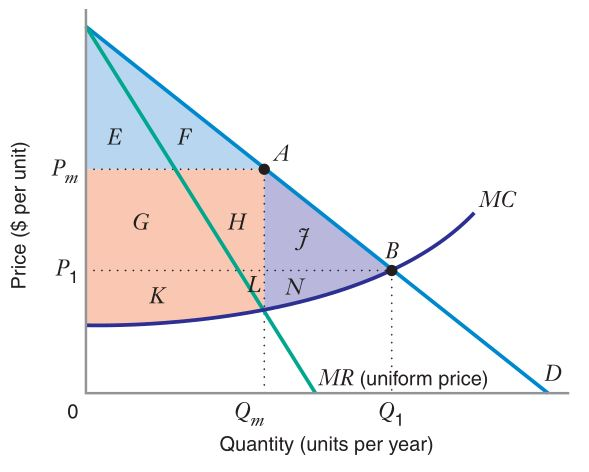
\includegraphics[width=220px]{figures/fig12_2a.jpg}
  \end{figure}
\end{frame}

\begin{frame}{First-Degree Price Discrimination}
  Would this work with a pair of designer sunglasses?

  \begin{itemize}
    \item Suppose the firm knew exactly how much each person that came into the store was willing to pay.
    
    \item And suppose that they charged every consumer their WTP.
  \end{itemize}
  
  \bigskip\pause
  Someone with a high WTP might instead just wait for someone with a low WTP to buy a pair and then offer them more than they paid

  \bigskip
  This illustrates why it can't be possible to resell the item. Otherwise, nobody would be willing to pay a higher price than anyone else.
\end{frame}

\begin{frame}{\bgCranberry{Try It Yourself}}
  Suppose a firm has constant marginal cost $MC = 2$, and faces a market demand curve of $P = 20 - Q$. 
  \only<1>{What will be a single-price monopolist's producer surplus in the market?} 
  \only<2>{Suppose that the firm can now perfectly price discriminate. What will be the firm's producer surplus?}
\end{frame}

\begin{frame}{First-Degree Price Discrimination}
  Higher education is a market where firms engage in first-degree PD. Even though universities are not monopolists, they still face a downward-sloping demand curve.

  \bigskip
  \emph{Question:} How do colleges estimate your WTP?

  \pause
  \begin{itemize}
    \item The price you pay depends on your expected family contribution (EFC) from FAFSA.
    
    \item Those with a higher ability to pay receive less money in need-based aid.
  \end{itemize}

\end{frame}

\begin{frame}{Second-Degree Price Discrimination}
  For many goods and services, consumers often buy more than one unit.

  \begin{itemize}
    \item And their individual demand curves are often downward sloping.
    
    \item In other words, their WTP decreases as they buy more.
    
    \item Sellers can capture additional surplus by charging customers a lower price for the second unit than the first.
  \end{itemize}

  \bigskip
  This is \textbf{second-degree price discrimination}
\end{frame}

\begin{frame}{Second-Degree Price Discrimination}
  The first form of second-degree PD is block pricing.

  \bigskip
  For example, suppose there is only one consumer in the market for electricity.

  \begin{itemize}
    \item The electric company charges \$11 per unit for the first 9 megawatt-hour used and \$8 for every Mwh after that.
    \item The consumer is will buy more than if every unit simply cost \$11, but the additional revenue can still be extracted for the first 9 units.
    \item This type of pricing is known as a \textbf{block tariff}.
  \end{itemize}
\end{frame}

\begin{frame}{Second-Degree Price Discrimination}
  The firm captures additional producer surplus by selling additional units at a lower price.
  \begin{figure}
    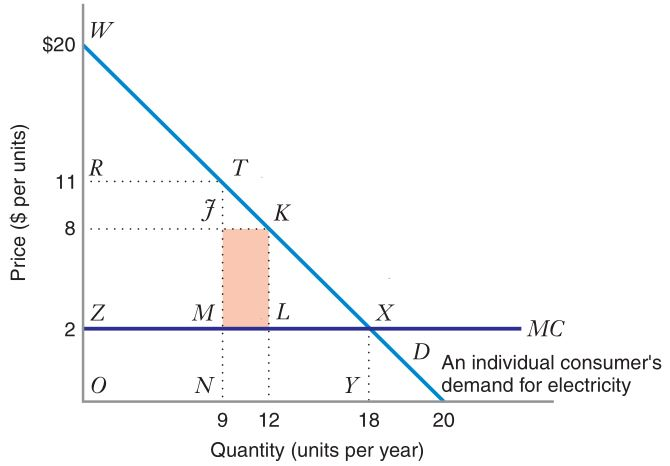
\includegraphics[width=220px]{figures/fig12_4.jpg}
  \end{figure}
\end{frame}

\begin{frame}{Second-Degree Price Discrimination}
  How do we find the optimal price and quantity for the first and second blocks?
  
  \begin{enumerate}
    \item Write producer surplus (or profit) in terms of $Q_1$ and $Q_2$.

    \item Maximize the profit function with respect to both $Q_1$ and $Q_2$. Find two equations.

    \item Solve the system of two equations for $Q_1$ and $Q_2$
  \end{enumerate}
\end{frame}

\begin{frame}{Second-Degree Price Discrimination}
  \begin{figure}
    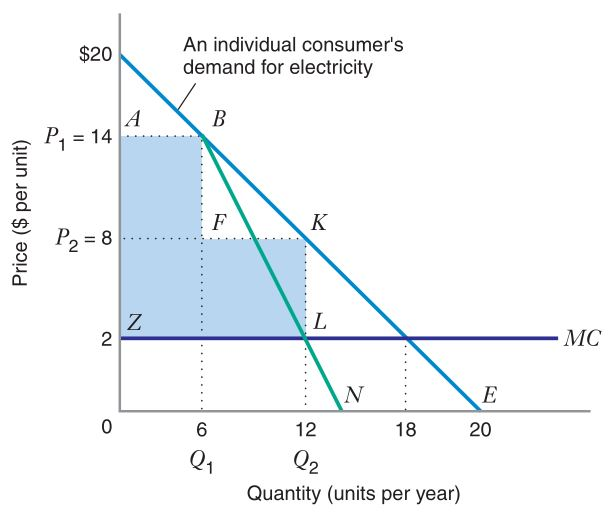
\includegraphics[width=220px]{figures/fig12_5.jpg}
  \end{figure}
\end{frame}

\begin{frame}{Second-Degree Price Discrimination}
  Example: Suppose demand is given by $P = 20 - Q$, and the firm's total cost is given by $TC(Q)=2Q$, such that $MC(Q)=2$.\\

  The firm's profit function is given by
  $$
    \Pi = P_1 Q_1 + P_2 (Q_2 - Q_1) - 2 * Q_2
  $$

  If we plug the demand function in for $P_1$ and $P_2$, we find
  $$
    \Pi = \underbrace{(20 - Q_1)}_{P_1 = P(Q_1)} Q_1 + \underbrace{(20 - Q_2)}_{P_2 = P(Q_2)} (Q_2 - Q_1) - 2 * Q_2
  $$
\end{frame}

\begin{frame}{Second-Degree Price Discrimination}
  We are solving an unconstrained maximization problem, so we simply take derivatives w.r.t. $Q_1$ and $Q_2$ and set equal to zero:
  \begin{align*}
    \frac{\partial}{\partial Q_1} & = (20 - 2Q_1) - 20 + Q_2 = 0 \\
    \frac{\partial}{\partial Q_2} & = 20 - 2Q_2 + Q_1 - 2 = 0
  \end{align*}

  \pause
  Simplifying the first equation, we have $Q_2 = 2 Q_1$. Plugging that into the second equation:
  \begin{align*}
    20 - 4Q_1 + Q_1 - 2 = 0 \implies Q_1^* = 6
  \end{align*}
\end{frame}

\begin{frame}{Second-Degree Price Discrimination}
  Plugging $Q_1^* = 6$ into the simplified first equation:
  $$
    Q_2^* = 12
  $$

  \bigskip
  Prices are found by plugging each quantity into the demand function:
  $$
    P_1^* = 20 - Q_1^* = 14 \qquad \text{and} \qquad P_2^* = 20 - Q_2^* = 8
  $$
\end{frame}

\begin{frame}{Second-Degree Price Discrimination}
  The second type of second-degree price discrimination is a two-part tariff.

  \begin{itemize}
    \item We discussed this from the consumer's perspective in chapter 5.
  \end{itemize}

  \bigskip
  A \textbf{two-part tariff} is when the firm charges a subscription fee, and then a per-unt price.

  \begin{itemize}
    \item Examples: Costco, Amazon Prime, Zipcar.
  \end{itemize}
\end{frame}

\begin{frame}{Second-Degree Price Discrimination}
  For example, suppose that a telephone company has a per-unit cost of \$0.05.

  \begin{itemize}
    \item If the provider sets the per-unit price to \$0.05, there will be no deadweight loss
    \item Then the firm can set the subscription cost to whatever price is needed to capture all of the surplus (e.g. \$20).
  \end{itemize}
\end{frame}

\begin{frame}{Second-Degree Price Discrimination}
  \begin{figure}
    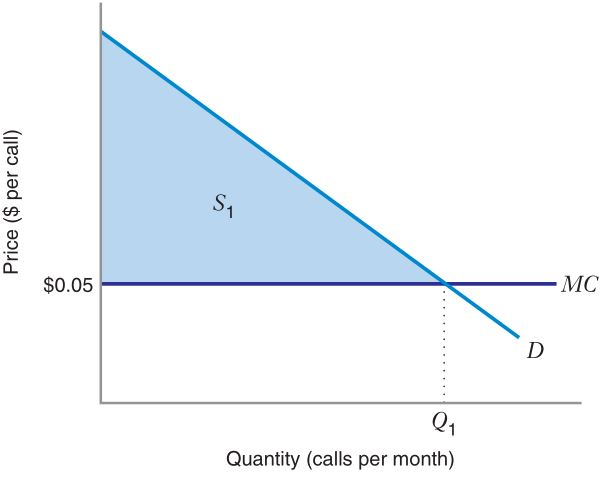
\includegraphics[width=180px]{figures/fig12_8.jpg}
  \end{figure}
\end{frame}

\begin{frame}{Second-Degree Price Discrimination}
  More generally, the firm should set the per-unit price such that $D = MC$ (as opposed to $MR = MC$).

  \begin{itemize}
    \item That's because with the subscription fee, they don't have to give up producer surplus on previous units.
    
    \item They just capture it back with the subscription fee.
    
    \item The subscription fee can be set as high as consumer surplus, and the consumer will be indifferent.
  \end{itemize}
\end{frame}

\begin{frame}{Second-Degree Price Discrimination}
  If there is a lot of heterogeneity in demand curves, then a firm can offer a menu of subscription packages.

  \begin{itemize}
    \item Think of a ski resort, or a cell phone service provider.
  \end{itemize}

  \bigskip
  Then the customers ``sort" themselves according to their demand.

  \begin{itemize}
    \item The firm can extract more surplus from each group.
  \end{itemize}
\end{frame}

\begin{frame}{Third-Degree Price Discrimination}
  Third-degree price discrimination means charging different prices to different groups of customers based on some observable characteristic. For example,
  \begin{itemize}
    \item Student prices at a movie theater
    \item Coupons and rebates
    \item Video game prices declining over time
  \end{itemize}

  \bigskip
  These allow the firm to charge higher prices to those with higher average willingness to pay.
\end{frame}

\begin{frame}{Third-Degree Price Discrimination}
  Consider rail transportation in the early 20th century:

  \begin{itemize}
    \item It cost the railroad about the same amount of money to transport coal and grain.
    
    \item But railroads faced more competition from barges and trucks when carrying grain (available substitutes)
    
    \item Thus, the railroad would charge 2-3 times the price to ship coal even though MC was the same
  \end{itemize}

  \bigskip Again, market power matters!
\end{frame}
 
\begin{frame}{Third-Degree Price Discrimination}
  The market demand for rail shipping is flatter for grain since there are better substitutes

  \bigskip
  \begin{figure}
    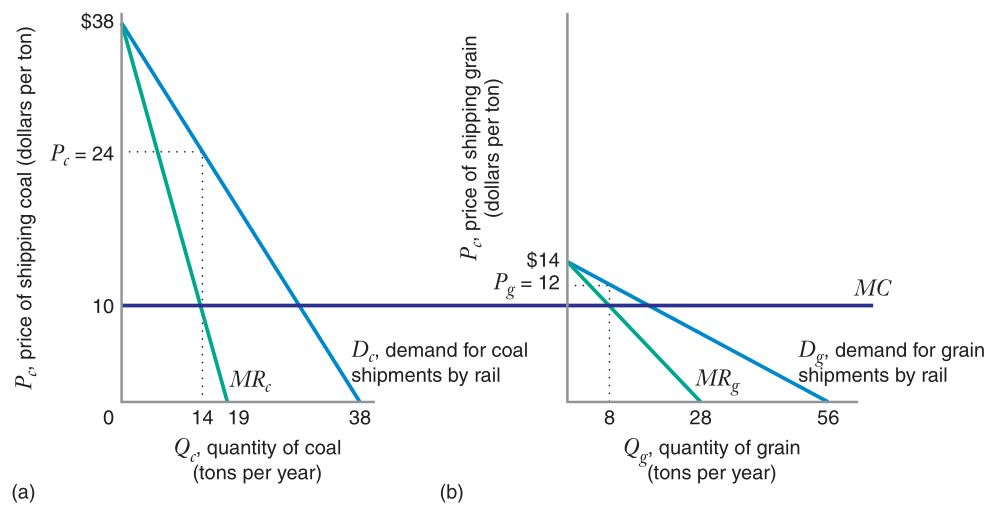
\includegraphics[width=280px]{figures/fig12_9.jpg}
  \end{figure}
\end{frame}

\begin{frame}{Third-Degree Price Discrimination}
  How does a firm decide the profit maximizing prices to charge?

  \begin{itemize}
    \item If $MC$ is constant, firm just sets $MR(Q^*) = MC(Q^*)$ in each market (or for each group), and then finds $P$ such that $D(P) = Q^*$ (just like single-price monopolist).
  \end{itemize}

  \bigskip\pause
  If $MC$ isn't constant, firm has to take into account that selling another unit in market $A$ increases the cost in market $B$. Firm's problem is:

  $$
    \max_{Q_A,Q_B} P_A Q_A + P_B Q_B + TC(Q_A + Q_B)
  $$
\end{frame}

\begin{frame}{Third-Degree Price Discrimination}
  Example: Suppose a railroad faces demand curves for transporting grain and coal given by $P_C = 38 - Q_C$ and $P_G = 14 - \frac{1}{4} Q_G$. Marginal cost is given by $MC=10$.
  \\

  For grain, the firm sets $MR(Q_G^*) = MC(Q_G^*$). $MR(Q_G^*)$ is given by
  $$
    \frac{\partial [P(Q_G) Q_G]}{\partial Q_G} = \frac{\partial [14 Q_G - \frac{1}{4} Q_G^2]}{\partial Q_G}  = 14 - \frac{1}{2} Q_G
  $$
\end{frame}

\begin{frame}{Third-Degree Price Discrimination}
  The optimal quantity of grain is given by:
  $$
    14 - \frac{1}{2}Q_G = 10 \implies Q_G^* = 8.
  $$

  Market price is
  $$
    P_G^* = 14 - \frac{1}{4} * 8 = 12
  $$
\end{frame}

\begin{frame}{Third-Degree Price Discrimination}
  For coal, the firm sets $MR(Q_C^*) = MC(Q_C^*$). $MR(Q_C^*)$ is given by
  $$
    \frac{\partial [P(Q_C) Q_C]}{\partial Q_C}= \frac{\partial [38Q_C - Q_C^2]}{\partial Q_C} =38-2Q_C
  $$
  The optimal quantity of coal is given by:
  $$
    38 - 2Q_C = 10 \implies Q_C^* = 14
  $$
  
  Market price is
  $$
    P_C^* = 38 - 14 = 24
  $$
\end{frame}

\begin{frame}{\bgCranberry{Try It Yourself}}
  Which of the following statements regarding a monopoly's first-degree price discrimination is correct?

  \begin{enumerate}[A)]
    \item With first-degree price discrimination, consumer surplus is small, yet still greater than zero.
    \item With first-degree price discrimination, producer surplus is lower than with uniform pricing.
    \item With first-degree price discrimination, deadweight loss is large.
    \item With first-degree price discrimination, total surplus is greater than when the monopoly charges a uniform price.
  \end{enumerate}
\end{frame}


\begin{frame}{Screening}
  Since it's so hard to know consumers' WTP, firms sometimes use observable characteristics to sort people into groups with high or low expected WTP.
  
  This is known as \textbf{screening}.

  \begin{itemize}
    \item For example, movie theaters figure that, on average, students have lower WTP.
    \item They can screen customers based on whether they are a student or not.
  \end{itemize}
\end{frame}

\begin{frame}{Intertemporal Price Discrimination}
  \textbf{Intertemporal price discrimination} is when a firm sells a good at different prices at different times of the day (or week, or year) to capture additional surplus.

  \begin{itemize}
    \item For example, movies and video games often sell at higher prices initially, and then the price falls over time.
    
    \item Airline tickets may be cheaper 3 months out, and very expensive one week out.    
  \end{itemize}
  
  \bigskip
  Note that prices declining over time does not always reflect price discrimination:
  \begin{itemize}
    \item Sometimes it's a result of decreasing marginal costs (think of flat-screen TVs)
    \item Sometimes it's a result of increasing competition in the market
  \end{itemize}
\end{frame}

\begin{frame}{Coupons and Rebates}
  Firms use coupons and rebates to price discriminate.

  \begin{itemize}
    \item People who are more price sensitive (lower WTP) are more likely to clip coupons
    \item They pay a lower net price as a result.
    \item Those who are less price sensitive may not bother with coupons.
  \end{itemize}
\end{frame}

\begin{frame}{Capacity Constraints}
  Some firms are constrained in the number of units of a good they can sell of a given product.

  \begin{itemize}
    \item Examples: Airlines, movie theaters, cruise lines.
  \end{itemize}

  \bigskip\pause 
  In that case, the firm may not be able to set $Q_1$ and $Q_2$ such that $MR(Q_1) = MC(Q)$ and $MR(Q_2) = MC(Q)$ where $Q = Q_1 + Q_2$.
  
  \bigskip
  Instead, suppose that $MR(Q_1) = MC(Q)$ but $MR(Q_2) > MC(Q)$ for two segments of some market.
  \begin{itemize}
    \item This implies $MR_2 > MR_1$
  \end{itemize}
\end{frame}

\begin{frame}{Capacity Constraints}
  If $MR_2 > MR_1$, what should the firm do?

  \begin{itemize}
    \item Since MC is the same for both market segments, we can focus only on MR.
  \end{itemize}
  
  \bigskip
  Recall that marginal revenue is the additional revenue from selling one more unit.

  \begin{itemize}
    \item Then if the firm sells one less unit in market 1 and one more unit market 2, total revenue will go up.
    \item Alternatively, if $MR_1>MR_2$, the firm should sell more to market 1 and less to market 2.
  \end{itemize}
\end{frame}

\begin{frame}{Capacity Constraints}
  Therefore, the optimal allocation to segments 1 and 2 is such that $MR_1 = MR_2$.

  \begin{itemize}
    \item Because of the capacity constraint, the firm can't produce enough to where $MR=MC$ for either segment.
  \end{itemize}

  \bigskip
  The result is that the firm must solve a system of two equations:

  $MR_1 = MR_2$ and $Q_1 + Q_2 = C$, where $C$ is the firm's capacity.
\end{frame}

\begin{frame}{Capacity Constraints}
  Do firms actually think about their problem in this way? Might seem somewhat unrealistic, but firms face this decision all the time

  \begin{itemize}
    \item Airlines have to decide where to set their prices so that they can sell some seats at a low price, and some at a higher price.
    \item Movie theaters have to decide how to set student and general admission prices to maximize profit.
  \end{itemize}
\end{frame}

\begin{frame}{Capacity Constraints}
  Suppose that a firm sells their good in two different markets, 1 and 2, and faces demand functions $Q_1 = 200 - 2P_1$ and $Q_2 = 250 - P_2$. Marginal cost is \$10 per unit, and the firm's capacity is 150 units. What is the optimal price and quantity in each market?

  \bigskip\pause
  The firm should set $Q_1$ and $Q_2$ such that $MR(Q_1) = MR(Q_2)$. Therefore, we need to find the marginal revenue curves for both segments.

  \bigskip
  First, write the demand functions such that P is a function of Q.
  $$
    P_1=100-\frac{1}{2}Q_1 \qquad \text{and} \qquad P_2=250 - Q_2
  $$
\end{frame}

\begin{frame}{Capacity Constraints}
  Next, find $MR_1$ and $MR_2$:
  \begin{align*}
    TR(Q_1) &= P_1*Q_1 = 100Q_1 - (1/2)Q_1^2 \implies MR(Q_1) = 100 - Q_1 \\
    TR(Q_2) &= P_2*Q_2 = 250Q_2 - Q_2^2 \implies MR(Q_2) = 250 - 2Q_2
  \end{align*}
  
  \bigskip
  Finally, equate $MR_1$ to $MR_2$, gives us $100 - Q_1 = 250 - 2Q_2$. Our capacity constraint is given by $Q_1 + Q_2 = 150$
\end{frame}

\begin{frame}{Capacity Constraints}
  Finally, we can solve this system of two equations. First, plug the second equation into the first:
  $$
    100 - (150 - Q_2) = 250 - 2Q_2 \implies Q_2^* = 100
  $$

  Then
  $$
    Q_1^* = 150 - Q_2^* = 150-100 = 50
  $$
  Finally, we can find prices using the segment demand functions:
  $$
    P_1^* = 100 - \frac{1}{2} 50 = 75 \qquad \text{and} \qquad P_2^* = 250 - 100 = 150
  $$
\end{frame}

\begin{frame}{\bgCranberry{Try It Yourself}}
  Let a monopolist face consumer group A with inverse demand $P_A = 100 - 2Q_A$ and consumer group B with inverse demand $P_B = 80 - Q_B$.  The monopolist can conduct third degree price discrimination, but faces a capacity constraint that $Q_A + Q_B \leq 50$. What will be the amount supplied to each of the customer groups?
\end{frame}

\begin{frame}
  
\end{frame}

\begin{frame}{Versioning}
  Another way that firms capture additional surplus is by versioning. \textbf{Versioning} is the strategy of selling two or more versions of a product with different qualities.

  \begin{itemize}
    \item For example, laptop manufacturers offer low-quality and high-quality versions of their products.
    
    \item The hope is that less price-sensitive consumers will be willing to pay a larger markup for the item with additional features, or quality.
    
    \item Likewise, the firm hopes that they can attract price sensitive consumers with a lower-quality product, without causing the price-insensitive consumers to switch.
  \end{itemize}


\end{frame}

\begin{frame}{Damaged Goods Strategy}
  An interesting type of versioning is known as the \textbf{damaged goods strategy}.

  \begin{itemize}
    \item A firm deliberately ``damages" a product by removing features or adjusting performance and sells that good to the low-WTP consumers.
    
    \item Ironically, damaging the product may create an additional cost, so that the damaged good has a higher MC.
  \end{itemize}
\end{frame}

\end{document}
